\newpage
\section[Basic Topology]{\hyperlink{toc}{Basic Topology}}
\subsection{Finite and Countable Sets}
This chapter is split into two portions; the first looks at counting, what it means for us to say that two sets have the same number of elements, and concludes with a classic theorem of Cantor concerning uncountable sets. The second part looks at the topology of metric spaces, before moving onto the topology of the real numbers. 

Let us then begin with our discussion of counting. If we consider counting how many bananas there are on a table (say there are 10 bananas), then what we are formally doing is establishing a correspondence between each ball on the table with an element in the set $\set{1, \ldots, 10}$. When we refer to the number of elements in a set, it will be good to keep in mind that we are establishing functions between sets. Although we have been discussing functions with some frequency in the course already, we give a definition below for completeness. 

\begin{definition}{Functions}{2.1}
    Let $A, B$ be sets. Then, a map that associates each element $x \in A$ with a unique element denoted as $f(x) \in B$ is a \textbf{function} $f: A \rightarrow B$. We then define $A$ as the \textbf{domain} of $f$ and the set $\set{f(x): x \in A}$ as the \textbf{range}. For $E \subset A$, we call $f(E) = \set{f(x): x \in E}$ the \textbf{image} of $E$ under $f$. For $F \subset B$, we call $f^{-1}(B) = \set{x \in A: f(x) \in B}$ the \textbf{preimage} of $F$. 
\end{definition}

\begin{definition}{Injective/Surjective Functions}{2.2}
    Let $f: A \mapsto B$ be a function. If for $x_1, x_2 \in A$ we have that $f(x_1) = f(x_2) \implies x_1 = x_2$ (or equivalently, $x_1 \neq x_2 \implies f(x_1) \neq f(x_2)$), then we say that $f$ is \textbf{injective}, or \textbf{one-to-one}. If for all $y \in B$ there exists $x \in A$ such that $y = f(x)$, then we say that $f$ is \textbf{surjective}, or \textbf{onto}. If a function is both injective and surjective, it is \textbf{bijective}.
\end{definition}
\noindent Intuitively, we can think of injectivity as implying each element in $B$ being reached at most once, and surjectivity implying that each element in $B$ is reached at least once. 

\begin{definition}{Cardinality \& Equivalence}{2.3}
    Let $A, B$ be sets. We say that $A, B$ have the same \textbf{cardinality} if there exists $f: A \mapsto B$ such that $f$ is bijective. We can denote this as $A \sim B$ where $\sim$ indicates an \textbf{equivalence relation}. An equivalence relation has three properties:
    \begin{enumerate}
        \item Reflexivity: $A \sim A$.
        \item Symmetry: If $A \sim B$ then $B \sim A$.
        \item Transitivity: If $A \sim B$ and $B \sim C$ then $A \sim C$.
    \end{enumerate}
    As a point of notation, $\abs{S}$ denotes the cardinality of the set $S$. 
\end{definition}

\noindent We get (a) from each set having a bijection to itself (i.e. the identity function), (b) from the fact that if there exists a bijection $f: A \mapsto B$, then there must exist an inverse $f^{-1}: B \mapsto A$, and (c) from if there exist bijections $f: A \mapsto B$ and $g: B \mapsto C$ then the composition $g \circ f: A \mapsto C$ will also be a bijection. 

\begin{definition}{Countability}{2.4}
    First, we denote $J_n = \set{1, 2, 3, \ldots, n}$ and $J = \NN = \set{1, 2, 3, \ldots}$. Let $A$ be a set. We say that $A$ is \textbf{finite} if it has a finite number of elements, that is, there exists $n \in \NN$ such that $A \sim J_n$. A set $A$ is \textbf{infinite} if it is not finite, and we cannot put $A$ in bijection with $J_n$ for any $n \in \NN$. We say that $A$ is \textbf{countable}if $A \sim \NN$, and \textbf{uncountable} otherwise. 
\end{definition}

\noindent Note that the above definition gives us a useful notion for what sets we can consider countable; if we can enumerate a set with the naturals, this yields a bijection with $\NN$ and hence the set must be countable. 

We here give some additional properties concerning cardinalities of sets, which may be useful:
\begin{itemize}
    \item $\abs{A} \leq \abs{B} \iff \exists f: A \mapsto B \text{ such that $f$ is injective}$
    \item $\abs{A} \geq \abs{B} \iff \exists f: A \mapsto B \text{ such that $f$ is surjective}$
    \item $\abs{A} \leq \abs{B} \text{ and } \abs{A} \geq \abs{B} \implies \abs{A} = \abs{B}$
\end{itemize}

\begin{example}{}{2.5}
    $\ZZ$ is countable. To see this, consider the function:
    \begin{align*}
        f = \begin{cases}
            \frac{n}{2} & \text{$n$ is even}
            \\ -\frac{n-1}{2} & \text{$n$ is odd}
            \end{cases}
    \end{align*}
    $f$ is a bijection (check!) and hence $\NN \sim \ZZ$. 
\end{example}
\noindent The above example serves as a bit of a warning sign. Even though $\NN \subsetneq \ZZ$ and $\ZZ$ has ``more elements'', we still find that the two sets have the same cardinality. A similar example is given by $\NN$ and the set of all even natural numbers (which we may denote $2\NN$); the bijection $f(n): n \mapsto 2n$ between these two sets shows that $\NN \sim 2\NN$, even though $2\NN$ is a strict subset of $\NN$. 
\setcounter{rudin}{7}

\begin{theorem}{}{2.8}
    A subset of a countable set is either finite or countable.
\end{theorem}
\begin{nproof}
    (Sketch) The countability of $A$ implies that $A = \set{a_1, a_2, a_3, a_4, a_5 \ldots}$ (in other words, we can enumerate the elements using $\NN$). Let $S \subset A$. Then, $S = \set{a_1, \cancel{a_2}, a_3, a_4, \cancel{a_5}, \ldots}$, that is, $A$ with some (or none) of the elements removed. Now, we can rename all the elements with $a_1, a_2, \ldots$; what we have left is again an enumeration, so it is yet again (at most) countable.
\end{nproof}
\noindent One potentially useful fact is that if we have a set $S$ and a function $f: \NN \mapsto S$ such that $f$ is surjective, then $S$ is at most countable. 

\begin{proof}
    Let $T = \set{n \in \NN: f(n) \neq f(m), \forall m = 1, 2, \ldots, m}$. We restrict $f: T \mapsto S$, then $f$ is injective by constructive. It is still surjective, hence $T \sim S$. Since $T \subset \NN$, by Theorem \ref{thm:2.8}, $S$ is finite or countable.
\end{proof}

\setcounter{rudin}{11}

\begin{theorem}{}{2.12}
    Let $E_1, E_2, \ldots$ be countable sets (i.e. we have a countable number of countable sets). Define $S = \bigcup_{n=1}^{\infty} E_n$. Then, $S$ is countable. 
\end{theorem}
\begin{nproof}
    Write $E_n = \set{x_{n1}, x_{n2}, x_{n3}, \ldots}$ (which we can do as each of the $E_n$s are countable). Then, we form an array:
    \begin{center}
    \begin{tikzpicture}
        \matrix[matrix of math nodes,inner sep=1pt,row sep=1em,column sep=1em] (M)
        {
            E_1 & = & x_{11} & x_{12} & x_{13}  & \cdots \\
            E_2 & = & x_{21} & x_{22} & x_{23}  & \cdots \\
            E_3 & = & x_{31} & x_{32} & x_{33}  & \cdots \\
            \cdots \\
        }
        ;
        \draw[->] (M-1-3.south west) -- (M-1-3.north east);
        \draw[->] (M-2-3.south west) -- (M-1-4.north east);
        \draw[->] (M-3-3.south west) -- (M-1-5.north east);
        \draw[->] (M-1-3.south west) -- (M-1-3.north east);
        \draw[->] (M-3-4.south west) -- (M-2-5.north east);
        \draw[->] (M-3-5.south west) -- (M-3-5.north east);
    \end{tikzpicture}
    \end{center}
    Then, we can re-number the elements along the diagonal lines (i.e. $x_{11}, x_{21}, x_{12}, x_{31}, x_{22}, x_{13}, \ldots$). This new enumeration corresponds to a countable set. From there, we let $T \subset \NN$ be the remaining labels in the enumeration after removing the repeated elements from the sequence. Then, $T \sim S$, and hence $S$ is at most countable. $S$ cannot be finite as $E_1 \subset S$ and $E_1$ is not finite. Hence $S$ is countable. \qed
\end{nproof}

\begin{corollary}{$\QQ$ is Countable.}{2.13}
    \begin{itemize}
        \item If $A$ is countable, the set of n-tuples of $(a_1, \ldots a_n)$ is also countable for any $n \in \NN$.  
        \item $\QQ$ is countable.
    \end{itemize}
\end{corollary}
\noindent We defined $\QQ$ as pairs of integers, but by the first part of the corollary (which follows immediately by application of Theorem \ref{thm:2.12}) $\ZZ^2$ (the set of pairs of integers) has equal cardinality to $\ZZ$, and since $\QQ$ is a subset of the set of pairs of integers, $\QQ$ is countable. 

Another way we can formalize this argument: if we let $X_t = \set{\frac{m}{n}: m \in \ZZ, n \in \NN, \abs{m} \leq t, n \leq t}$, then we have that $\abs{X_t}$ is at most $t\cdot (2t+1)$ (the first term being the choises for $n$, the second term being the choices for $m$). Of course, the cardinality of $X_t$ is actually less than that as we would have to remove repeats. Nontheless, we have that $\QQ = \bigcap_{t=1}^\infty X_t$ and hence $\QQ$ would be countable by Theorem $\ref{thm:2.12}$. 

From the discussion of today, we have established that $\abs{\NN} = \abs{\ZZ} = \abs{\QQ}$. Does $\RR$ also have equal cardinality to these sets? Do infinite sets in general have the same cardinality? The answer turns out to be no for both of these questions. We will answer the first question in the next lecture (when we discuss Cantor diagonalization, a highlight of the course), but we can discuss the second statement now. First, we make a definition:
\begin{ndef}{: Power Sets}
    Let $A$ be a set. Then, the \textbf{power set} of $A$, denoted $\mathcal{P}(A)$, is the set of all subsets of $A$. 
\end{ndef}
\noindent An interesting theorem then follows:
\begin{ntheorem}{: Power Set Cardinality}
    Let $A$ be a set. Then, $\abs{A} < \abs{\mathcal{P}(A)}$.
\end{ntheorem}
\begin{nproof}
    Suppose for the sake of contradiction that there exists a surjection $f: A\rightarrow \pset{A}$ (this would imply that $\abs{A} \geq \abs{\pset{A}}$, so by showing this is false, we obtain the desired result). Then, each element $x \in A$ gets mapped to some subset of $A$. We either have that $x$ belongs to the subset that it gets mapped to, or it doesn't. Therefore, we can define a new subset $B \subset A$, such that:
    \[B = \set{x\in A: x \notin f(x)}\]
    In other words, the set of all $x$s that are not in the subset that they get mapped to by $f$. Since $f$ is surjective, there must be an element $y \in A$ such that $f(y) = B$. One of $y \in B$, $y \notin B$ must be true. If $y \in B$, by construction of $B$ we have that $y$ is not in the subset that it gets mapped to by $f$, which is a contradiction. If $y \notin B$, by definition of $B$, $y \in B$ as it is not in the subset that it gets mapped to, yet again a contradiction. Therefore, we conclude that no $y \in A$ exists such that $f(y) = B$, and hence, no surjective $f$ exists such that $f: A \rightarrow \pset{A}$. Hence, $\abs{A} < \abs{\pset{A}}$. \qed
\end{nproof}
\noindent An interesting consequence of this theorem is that for a countable set $A$, we then have that $\mathcal{P}(A)$ is an infinite set which has greater cardinality! For example, $\abs{\NN} < \abs{\mathcal{P}(\NN)}$. Moreover, this gives rise to an infinite number of cardinalities in ascending order; $\abs{\NN} < \abs{\pset{\NN}} < \abs{\pset{\pset{\NN}}} < \cdots$ and so on.

\subsection{Uncountable Sets}
\begin{theorem}{Existence of Uncountable Sets}{2.14}
Let $A = \set{(b_1, b_2, \ldots), b_n \in \set{0, 1}}$ be the set of binary sequences. Then, $A$ is uncountable. 
\end{theorem}
\begin{nproof}
    It suffices to show that every countable subset of $A$ is a proper subset of $A$. Let $E \subset A$ be countable, and let $E = \set{S^{(1)}, S^{(2)}, S^{(3)}, \ldots}$. To show that $E$ is a proper subset, we show that there exists a sequence $S \in A \setminus E$. To construct such an $S$, let us put the elements of $E$ in an array. 
    \begin{center}
        \begin{tikzpicture}
            \matrix[matrix of math nodes,inner sep=1pt,row sep=1em,column sep=1em] (M)
            {
                S^{(1)} & = & \boxed{b_{1}^{1}} & b_{2}^{1} & b_{3}^{1} &  \cdots \\
                S^{(2)} & = & b_{1}^{2} & \boxed{b_{2}^{2}} & b_{3}^{2} & \cdots \\
                S^{(3)} & = & b_{1}^{3} & b_{2}^{3} & \boxed{b_{3}^{3}}  & \cdots \\
            };
        \end{tikzpicture}
    \end{center}
    Then, define:
    \[\tilde{b}_n^n = \begin{cases}
        1 & \text{if $b_n^n = 0$}
        \\ 0 & \text{if $b_n^n = 1$}
    \end{cases}\]
    I.e. $\tilde{b}_n^n$ is the bit flip of $b_n^n$. Then, let $S = (\tilde{b}_1^1, \tilde{b}_2^2, \tilde{b}_3^3, \ldots)$, that is, $S$ is the sequence of bit-flipped diagonal elements of the original array. By construction, $S \neq S^{(k)}$ as for any $S^{(k)} \in E$ as $S$ differs at the $k$th position. Hence, $S \notin E$ and therefore $E \subsetneq A$. \qed
\end{nproof}
\noindent The above proof is a very famous argument, invented by the mathematician George Cantor. The discovery that there exist sets with greater cardinality than $\NN$ was initially quite controversial in the math community!

\begin{ncorollary}{: $\RR$ is Uncountable}{}
    $\mathcal{P}(\NN)$ (the power set of $\NN$) is uncountable. $\RR$ is uncountable.
\end{ncorollary}
\begin{nproof}
    Although we showed that $\mathcal{P}(\NN)$ was uncountable last lecture, we show this in an alternative way by considering a bijection between $\mathcal{P}(\NN)$ and the set $A$ of binary sequences. To do this, consider that we can associate a subset $T \subset \NN$, $T \in \mathcal{P}(\NN)$ with the sequence corresponding to:
    \begin{align*}
        b_n = \begin{cases}
            1 & \text{if $n \in T$}
            \\ 0 & \text{if $n \notin T$}
        \end{cases}
    \end{align*}
    Since $A$ is uncountable, it follows that $\mathcal{P}(\NN)$ is uncountable. The second statement in the corollary follows (roughly) by considering $\RR$ represented in binary, though this requires more justification than what we present here (we will show below that a subset of $\RR$ is uncountable). \qed
\end{nproof}
\begin{ntheorem}{}{}
    $[0, 1] \subset \RR$ is uncountable.
\end{ntheorem}
\begin{nproof}
    (Sketch) We construct a bijection from $[0, 1]$ to $A$. Let $x \in [0,1]$, and let $b_1$ be the largest integer such that $N_1 = \frac{b_1}{2} \leq x$. Then, let $b_2 \in \set{0, 1}$ be the largest integer such that $N_2 = \frac{b_1}{2} + \frac{b_2}{2^2} \leq x$. We can continue dividing $[0,1]$ in half in this way, approximating $x$ by powers of 2 (a decimal expansion in binary). Then, let $E(x) = \set{N_1, N_2, N_3, \ldots}$. By construction, $E(x)$ is bounded above by $x$ and nonempty. Hence, $\sup(E(x))$ exists and is unique, and in fact is equal to $x$ (note that we are in essence constructing an "infinite series" where the sequence of partial sums is increasing and bounded, approaching $x$ from the left). Doing this we can associate $(b_1, b_2, b_3, \ldots) \in A$ with every number $x \in [0, 1]$ and therefore $[0, 1] \sim A$. Hence $[0, 1]$ is uncountable. \qed
\end{nproof}
\noindent It might be worth investigating why a more naive approach to the above argument may fail. Let $D$ be the sets of all decanary sequences, i.e. all sequeces of the form $(d_1, d_2, d_3, \ldots)$ where $d_n \in \set{n \in \ZZ, 0 \leq n \leq 9}$. Then, it might be tempting to say that the function:
\begin{align*}
    \fullfunction{f}{D}{[0, 1]}{(d_1, d_2, d_3, \ldots)}{0.d_1d_2d_3\ldots}
\end{align*}
Is a bijection; however, it is actually not the case! To see this, consider that $0.1000\ldots = 0.0999\ldots$. The sequences $(1, 0, 0, 0, \ldots)$ and $(0, 9, 9, 9, \ldots)$ are distinct, but the real number they would map to would be the same. This map is not an injection but a surjection. To show that $\RR$ is uncountable, we require an injection from $D$ to $[0, 1]$. So instead, what we have done with the above proof is map the set of binary sequences $B$ to $[0, 1]$:
\begin{align*}
    \fullfunction{g}{B}{[0, 1]}{(b_1, b_2, b_3, \ldots)}{\sum_{j=1}^\infty b_j 3^{-j} = \sup\set{\sum_{j=1}^N b_j3^{-j}: N \in \NN}}
\end{align*}
Note that in general, an infinite sum is not equal to the supremum of its partial sums (as a counterexample, consider the sum with first term 1, the second term -1, and all the remaining terms 0; evidently the value of the infinite sum is 0, but the supremum of the partial sums would be 1.) We will define an infinite sum more generally in chapter 3, but in our case here, this definition suffices as in the case where all terms of the sum are non-negative, the supremum of the partial sums is indeed the value of the infinite sum. We leave it as an exercise to show that $g$ is an injection. Also, one neat remark; the above set is equivalent to the Cantor set, which we will more formally define/discuss in Chapter 2. 

We take note a theorem that if $Y$ is a set, and there exists $X \subset Y$ such that $X$ is in bijective correspondence with an uncountable set, then $Y$ is also uncountable. Thus we can use the above theorem to conclude that $\RR$ is uncountable.

\subsection{Topology of Metric Spaces}
In our investigation of topology, we will try to better understand distances between and neighbourhoods of points. To do so, we first introduce the notion of a metric space.
\begin{definition}{Metric Spaces}{2.15}
    A set $X$ is a \textbf{metric space} (whose elements we call points) with a \textbf{metric} $d: X \times X \mapsto \RR$ such that for $x, y, z \in X$:
    \begin{enumerate}
        \item $d(x, y) > 0$ if $x \neq y$; $d(x, x) = 0$;
        \item $d(x, y) = d(y, x)$ ($d$ is symmetric);
        \item $d(x, z) \leq d(x, y) + d(y, z)$ (triangle inequality).
    \end{enumerate}
\end{definition}
\begin{example}{}{2.16}
    $\NN, \QQ, \RR, \RR^n, \CC$ are all metric spaces with $d(x, y) = \abs{x - y}$. Any subset $Y \subset X$ of a metric space is also a metric space, with the same metric. 
\end{example}
\noindent Another example of a metric space is given below; note that this example can be generalized, in that any connected graph can be made into a metric space. 
\begin{figure}[htbp]
    \centering
    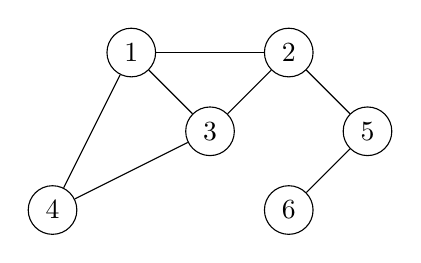
\begin{tikzpicture}
        \node[circle, draw] (1) at (0, 0) {1};
        \node[circle, draw] (2) at (2, 0) {2};
        \node[circle, draw] (3) at (1, -1) {3};
        \node[circle, draw] (4) at (-1, -2) {4};
        \node[circle, draw] (5) at (3, -1) {5};
        \node[circle, draw] (6) at (2, -2) {6};
        \draw[] (1) -- (2);
        \draw[] (1) -- (3);
        \draw[] (1) -- (4);
        \draw[] (2) -- (3);
        \draw[] (2) -- (5);
        \draw[] (3) -- (4);
        \draw[] (5) -- (6);
    \end{tikzpicture}
    
    \caption{A graph-theoretic example of a metric space. Let $X = \set{1, 2, 3, 4, 5, 6}$. Then, for $x, y \in X$, let $d(x, y)$ be the number of edges if the shortest path between $x$ and $y$. Properties (a), (b) of a metric are immediately satisfied, and (c) follows from the property of the shortest path.}
    \label{fig5}
\end{figure}

\noindent It may be of interest to consider other possible metrics. The discrete metric is defined such that $d(x, y) = 1$ if $x \neq y$ and $d(x, x) = 0$. The L1 Norm is defined such that $d(f, g) = \int_0^1 \abs{f(x) - g(x)} dx$ where $f, g$ are functions. In an inner product space, we have that $d(v, w) = \norm{v - w} = \avg{v-w, v-w}^{1/2}$; if $v, w$ are functions, then we have that $d(v, w) = \left(\int_0^1\abs{v(x) - w(x)}^2 dx\right)^{1/2}$. In analysis, we are often interested in the notion of things being \textunderscore{close} to other things (e.g. with limits, continuity) so a notion of distance is extremely important to define.

\setcounter{rudin}{17}
\begin{definition}{Neighbourhoods}{2.18a}
    A \textbf{neighbourhood} in a metric space $X$ is a set $N_r(p) = \set{q \in X: d(p, q) < r}$ with $r > 0$. 
\end{definition}

\begin{nexample}{}
    \begin{itemize}
        \item In $\RR$, $N_r(p)$ is the interval $(p - r, p + r)$ about midpoint $p$.
        \item In $\RR^2$, $N_r(p)$ is the open disk about center $p$. 
        \item In $\RR^3$, $N_r(p)$ is the open ball about center $p$.
        \item In $\RR^n$, $N_r(p)$ is the open hyperball about center $p$. 
    \end{itemize}
\end{nexample}
\noindent As another example, consider that in $\ZZ$, $N_1(0) = \set{0}, N_{3/2} = \set{-1, 0, 1}$ and $N_2(0) = \set{-1, 0, 1}$.
\setcounter{rudin}{17}

\begin{definition}{Interior Points}{2.18e}
    Let $E \subset X$. Then, $p$ is an \textbf{interior point} of $S$ if there is a neighbourhood $N_r(p)$ such that $N \subset E$. 
\end{definition}
\noindent Intuitively, an interior point of $E$ is a point that is not on the boundary of $E$. As an example, in $\RR^n$, if $E = \set{y: \abs{x - y} \leq 1}$, then the interior points of $E$ (which we can denote as $E^\circ$) are $E^\circ = \set{y: \abs{x - y} < 1}$. The idea is that there is always some finite distance to the boundary, so we can always fit a (perhaps small) open ball in. But this doesn't hold at the boundary!
\begin{figure}[htbp]
    \centering
    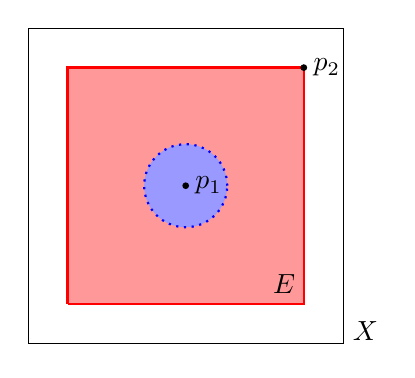
\begin{tikzpicture}
        \draw[] (-2, -2) -- (-2, 2) -- (2 ,2) -- (2, -2) -- (-2, -2);
        \draw[red, thick, fill = white!60!red] (-1.5, -1.5) -- (-1.5, 1.5) -- (1.5, 1.5) -- (1.5, -1.5) -- (-1.5, -1.5);
        \draw[blue, dotted, thick, fill = white!60!blue] (0, 0) circle (15pt);
        \draw[fill] (1.5, 1.5) circle (1pt);
        \draw[fill] (0, 0) circle (1pt);
        \node[right] at (0, 0) {$p_1$};
        \node[right] at (1.5, 1.5) {$p_2$};
        \node[] at (1.25, -1.25) {$E$};
        \node[right] at (2, -1.85) {$X$};
    \end{tikzpicture}
    \caption{A visualation of an interior point. A set $E \subset X$ is pictured. $p_1$ is an interior point as there exists $N_r(p_1) \subset E$. $p_2$ is not an interior point as there does not exist a neighbourhood of $p_2$ that is entirely contained in $E$ (it is on the boundary). }
    \label{fig6}
\end{figure}

\newpage 
\setcounter{rudin}{17}
\begin{definition}{Open Sets}{2.18f}
    A set $E \subset X$ is \textbf{open} if every point of $E$ is an interior point of $E$. 
\end{definition}

\begin{theorem}{}{2.19}
    Every neighbourhood is an open set.
\end{theorem}
\begin{nproof}
    Consider a neighbourhood $E = N_r(p) \subset X$. Let $q \in E$. We will show that $q$ is an interior point of $E$. Choose $s < r - d(p, q)$. Then, let $x \in N_s(q)$. By the triangle inequality:
    \begin{align*}
        d(x, p) \leq d(x, q) + d(q, p) < s + d(q, p) < r - d(p, q) + d(p, q) = r.
    \end{align*}
    Hence, $d(x, p) < r$ and it follows that $x \in N_r(p)$. Hence, $N_s(q) \subset N_r(p)$ and $q$ is an interior point of $E$. \qed
\end{nproof}

\begin{figure}[htbp]
    \centering
    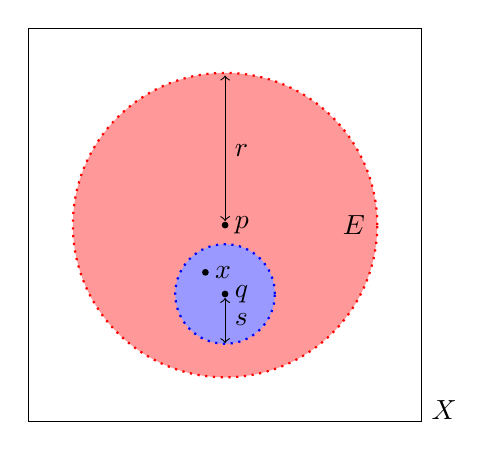
\begin{tikzpicture}
        \draw[red, dotted, thick, fill = white!60!red] (0, 0) circle (55pt);
        \draw[fill] (0, 0) circle (1pt);
        \node[right] at (0, 0) {$p$};
        \node[right] at (0, 0.95) {$r$};
        \draw[<->] (0, 0.05) -- (0, 1.9);
        \node[left] at (1.9, 0) {$E$};
        \draw[blue, dotted, thick, fill = white!60!blue] (0, -0.875) circle (18pt);
        \draw[fill] (0, -0.875) circle (1pt);
        \node[right] at (0, -0.875) {$q$};
        \draw[<->] (0,-0.925) -- (0, -1.5);
        \node[right] at (0, -1.2) {$s$};
        \draw[fill] (-0.25, -0.6) circle (1pt);
        \node[right] at (-0.25, -0.6) {$x$};
        \draw[] (-2.5, -2.5) -- (-2.5, 2.5) -- (2.5, 2.5) -- (2.5, -2.5) -- (-2.5, -2.5);
        \node[right] at (2.5, -2.35) {$X$};

    \end{tikzpicture}
    \caption{Visualization of the Sets/Points in Theorem \ref{thm:2.19}}
    \label{fig7}
\end{figure}

\setcounter{rudin}{17}
\begin{definition}{Limit Points/Isolated Points}{2.18b}
    Let $E \subset X$ and $p \in X$. Then, $p$ is a \textbf{limit point} of $E$ if every neighbourhood of $p$ contains $q \in E$, $q \neq p$. If $p \in E$ and $p$ is not a limit point of $E$, then $p$ is an \textbf{isolated point} of $E$. 
\end{definition}
\begin{nexample}{}{}
    Let $E = \set{\frac{1}{n}: n \in \NN}$. Then, $\frac{1}{2}$ is not a limit point of $E$, as for $r < \frac{1}{4}$ $N_r(\frac{1}{2})$ does not contain any other points of $E$. On the other hand, $0$ is a limit point of $E$. For any neighbourhood $N_r(0)$ of $0$, $\frac{1}{N} \in N_r(0)$ for $N > \frac{1}{r}$. Note that $0$ is the only limit point of $E$, and is not contained in $E$ (indeed, there is no requirement that a limit point be contained in the set). 
\end{nexample}

\setcounter{rudin}{19}

\begin{theorem}{}{2.20}
    If $p$ is a limit point of $E$, then every neighbourhood of $p$ contains an infinite number of $q \in E$. 
\end{theorem}

\begin{nproof}
    (Sketch) Let $r_1 = 1$. Then, there exists $q_1 \in N_{r_1}(p)$ such that $q_1 \in E$ and $q_1 \neq p$ as $p$ is a limit point of $E$ by assumption. Let $r_2 = d(q_1, p)$. Then, there exists $q_2 \in N_{r_2}(p)$ such that $q_2 \in E$ and $q_2 \neq p$. We can repeat this process to get a (countably infinite) sequence of distinct points $q \in N_{r_1}(p)$, which proves the claim. \qed 
\end{nproof}

\begin{ncorollary}{}{}
    If $E \subset X$ is finite, then $E$ has no limit points.
\end{ncorollary}

\setcounter{rudin}{17}
\begin{definition}{Dense Sets}{2.18j}
    $E \subset X$ is dense in $X$ if every point of $X$ is a limit point of $E$, or a point of $E$.
\end{definition}
\noindent By consequence of Theorem \ref{thm:1.20}, we have that $\QQ$ is dense in $\RR$ and $\RR \setminus \QQ$ is dense in $\RR$. As a general method to show that a set is dense in another set, take $x \in X \setminus E$, and show $x$ must be a limit point of $E$.

\setcounter{rudin}{17}
\begin{definition}{Bounded Sets}{2.18i}
    $E \subset X$ is bounded if there exists $M \in \RR$ and a point $q \in X$ such that $d(p, q) < M$ for all $p \in E$.
\end{definition}
\noindent For example, $(0, 1), [0, 1], [0, 1] \times [0, 1]$ are bounded, and $(0, \infty), \NN, \RR$ are unbounded (with the usual metric on $\RR$). 

\setcounter{rudin}{17}
\begin{definition}{Closed Sets}{2.18d}
    A set $E \subset X$ is closed if every limit point of $E$ is in $E$. 
\end{definition}
\noindent Note that with the above Corollary, we find that every finite set is (trivially) closed.

\setcounter{rudin}{17}
\begin{definition}{Complement}{2.18g}
    Let $E \subset X$. Then, the complement of $E$, denoted $E^c$ is $E^c = \set{x \in X: x \notin E}$. 
\end{definition}
\begin{figure}[htbp]
    \centering
    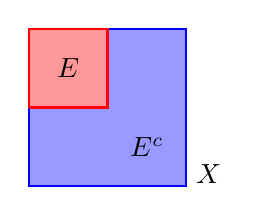
\begin{tikzpicture}
        \draw[] (-1, -1) -- (1, -1) -- (1, 1) -- (-1, 1) -- (-1, -1);
        \draw[blue, thick, fill = white!60!blue] (-1, 0) -- (-1, -1) -- (1, -1) -- (1, 1) -- (0, 1) -- (0, 0) -- (-1, 0);
        \draw[red, thick, fill = white!60!red] (-1, 0) -- (0, 0) -- (0, 1) -- (-1, 1) -- (-1, 0);
        \node at (-0.5, 0.5) {$E$};
        \node at (0.5, -0.5) {$E^c$};
        \node[right] at (1, -0.85) {$X$};
    \end{tikzpicture}
    
    \caption{Visualization of a set $E$ and its complement.}
    \label{fig8}
\end{figure}

\setcounter{rudin}{22}
\begin{theorem}{}{2.23}
    A set $E \subset X$ is open if and only if $E^c$ is closed.
\end{theorem}
\noindent Note that this theorem does not imply that all sets are closed or open; it is possible to have a set that is neither closed or open (such as $[0, 1) \subset \RR$) and then its complement (with the former example, $(-\infty, 0) \cup [1, \infty)$) which is also neither closed nor open (indeed, most sets are neither closed nor open). As an additional note, we have that $X$ (the entire metric space) and $\emptyset$ are both open and closed (which we may affectionately label as ``clopen'').

\begin{nproof}
    \boxed{\implies} Assume $E$ is open. If $E^c$ has no limit points, it is trivially closed, so suppose that there exists a limit point $x$ of $E^c$. Suppose for the sake of contradiction that $x \notin E^c$. Then, $x \in E$. As $E$ is open, $x$ is an interior point of $E$, so there exists a neighbourhood $N_r(x) \subset E$. In particular, $N_r(x) \cap E^c = \emptyset$, contradicting the fact that $x$ is a limit point of $E^c$. Hence, $x \in E^c$ and $E^c$ is closed.

    \boxed{\impliedby} Assume $E^c$ is closed. Let $x \in E$. In particular, $x \notin E^c$, so $x$ is not a limit point of $E^c$. So, there exists a neighbourhood $N_r(x)$ which contains no point of $E^c$, i.e. $N_r(x) \cap E^c = \emptyset$. It follows that $N_r(x) \subset E$, and hence $x$ is an interior point of $E$. This argument applies to all points of $E$, hence $E$ is open. \qed
\end{nproof}

\begin{ncorollary}{}{}
    A set $F \subset X$ is closed if and only if $F^c$ is open.
\end{ncorollary}
\noindent Let $F = E^c$ in Theorem \ref{thm:2.23} to realize the above Corollary.

\begin{theorem}{}{2.24}
    \begin{enumerate}
        \item For any collection $\set{E_\alpha}$ of open sets, $\bigcup_\alpha E_\alpha$ is open.
        \item For any collection $\set{F_\alpha}$ of closed sets, $\bigcap_\alpha F_\alpha$ is closed.
        \item For any finite collection $E_1, \ldots, E_n$ of open sets, $\bigcap_{i=1}^n E_i$ is open.
        \item For any finite collection $F_1, \ldots, F_n$ of closed sets, $\bigcup_{i=1}^n F_i$ is closed.
    \end{enumerate}
\end{theorem}
\noindent A point of notation; $\set{E_\alpha}$ can be finite, countable, or uncountable; the indices $\alpha$ are taken from an index set $A$ which can be chosen to be of any cardinality. 
\begin{nproof}
    \begin{enumerate}
        \item Suppose all sets in $\set{E_\alpha}$ are closed. Let $x \in \bigcup_{\alpha}E_\alpha$. Then, there exists $\alpha_0$ such that $x \in E_{\alpha_0}$. Since $E_{\alpha_0}$ is open, there exists a neighbourhood $N_r(x)$ of $x$ such that $N_r(x) \subset E_{\alpha_0} \subset \bigcup_{\alpha} E_\alpha$. Hence, $\bigcup_{\alpha} E_\alpha$ is open.
        \item Suppose all sets in $\set{F_\alpha}$ are open. To show that $\bigcap_\alpha F_\alpha$ is closed, we show that $\left(\bigcap_\alpha F_\alpha\right)^c$ is open (by Theorem \ref{thm:2.23}). We have that $\left(\bigcap_\alpha F_\alpha\right)^c = \bigcup_\alpha F_\alpha^c$. As all $F_\alpha^c$ are open, by part (a) we have that $\bigcup_\alpha F_\alpha^c$ is also open. Hence $\bigcap_\alpha F_\alpha$ is closed.
        \item Suppose $E_1,\ldots, E_n$ are open. Let $x \in \bigcap_{i=1}^n E_i$, and then we have that $x \in E_i$ for all $i \in \set{1, \ldots, n}$. Hence, there exists $r_i$ such that $N_{r_i}(x) \subset E_i$ as each of the $E_i$s are open. Let $r = \min\set{r_1, \ldots, r_n}$ and then we have that $N_r(x) \subset N_{r_i}(x) \subset E_i$ for all $E_i$. Therefore, $N_r(x) \subset \bigcap_{i=1}^n E_i$ and $\bigcap_{i=1}^n E_i$ is open.
        \item Suppose $F_1, \ldots, F_n$ are closed. By Theorem \ref{thm:2.23} we have that $\bigcup_{i=1}^n F_i$ is closed if and only if $\left(\bigcup_{i=1}^n F_i\right)^c = \bigcap_{i=1}^n F_i^c$ is open. Since all $F_i^c$s are open, by part (c) $\bigcap_{i=1}^n F_i^c$ is open, and hence $\bigcup_{i=1}^n F_i$ is closed. \qed
    \end{enumerate}
\end{nproof}

\begin{example}{}{2.25}
    We consider some examples to see why the finiteness of the collections in parts (c)/(d) of the theorem are essential. Suppose $E_n = \left(-\frac{1}{n}, \frac{1}{n}\right) \subset \RR$. These sets form a countably infinite collection of subsets of $\RR$. We then consider that $\bigcap_{n=1}^\infty E_n = \set{0}$, which is not open; showing that openness is not preserved under infinite intersections. Next, consider $F_n = [0, 1-\frac{1}{n}] \subset \RR$, which form a countably infinite collection of closed sets in $\RR$. We then have that $\bigcup_{n=1}^\infty F_n = [0, 1)$ which is not closed as $0$ is not an interior point of the set. Hence, closedness is not preserved under infinite unions. 
\end{example}

\subsection{Closure and Relative Topology}
As a review of some definitions of the previous section, we call a set open if every point of the set is an interior point, and closed if it contains all of its limit points. A complement of an open set is closed and vise versa. We also note that openness is preserved under infinite unions and finite intersections, and closedness is preserved under infinite intersections and finite unions. 

\begin{definition}{Closure}{2.26}
    Let $X$ be a metric space. Let $E \subset X$, and denote $E'$ as the set of all limit points of $E$. Then, the set $\overline{E} = E \cup E'$ is the \textbf{closure} of $E$.
\end{definition}

\begin{theorem}{}{2.27}
    \begin{enumerate}
        \item $\overline{E}$ is closed.
        \item $E = \overline{E}$ if and only if $E$ is closed.
        \item $\overline{E} \subset F$ for every closed set $F \subset X$ such that $E \subset F$.
    \end{enumerate}
\end{theorem}
\begin{nproof}
    \begin{enumerate}
        \item Let $p \in \overline{E}^c = E^c \cap (E')^c$. Then, $p \notin E$, and furthermore $p \notin E'$ so $p$ is not a limit point of $E$. Hence, there exists a neighbourhood $N_r(p)$ such that $N_r(p) \cap E = \emptyset$. Moreover, no point of $N_r(p)$ is in $E'$ (if there existed $q \in E'$ such that $q \in N_r(p)$, then there would exist some $N_{r'}(q)$ (which contains points of $E$) such that $N_{r'}(q) \subset N_r(p)$ which contradicts the fact that $N_r(p)$ contains no points of $E$). Hence, $N_r(p) \subset E^c \cap (E')^c = \overline{E}^c$. Hence, $\overline{E}^c$ is open and $\overline{E}$ is closed.
        \item $\boxed{\implies}$ If $E = \overline{E}$, then $E$ is closed by (a).
        
        $\boxed{\impliedby}$ If $E$ is closed, then $E$ contains all of its limit points, so $\overline{E} = E \cup E' \subset E$. By definition $\overline{E} \supseteq E$, so $E = \overline{E}$. 
        \item Let $E \subset F$ with $F$ closed. Then, $F' \subset F$. Also, $E' \subset F'$. So, by (b) we have $F = \overline{F} = F \cup F' \supseteq E \cup E' = \overline{E}$. \qed
    \end{enumerate}
\end{nproof}

\noindent We will soon define the notion of being relatively open, but before doing so, we consider a motivating example.

\begin{figure}[htbp]
    \centering
        \begin{tikzpicture}
            \draw[latex-latex,very thick] (-2,0)--(2,0);
            \draw[latex-latex,very thick] (0,-2)--(0,2); 
            \node[] at (0.5,0) {$($};
            \node[above] at (0.5, 0.1) {$a$};
            \node[] at (1.5,0) {$)$};
            \node[above] at (1.5, 0.1) {$b$};
            \node[] at (1.6, 1.6) {$\RR^2$};
        \end{tikzpicture}
    \caption{The interval $(a, b)$ embedded in $\RR^2$.}
    \label{fig9}
\end{figure}
In $\RR$, we know $(a, b)$ to be in an open set. However, embedded in $\RR^2$, $(a, b)$ has no interior points; any neighbourhood about any $x \in (a, b)$ extends into the plane and will inevitably contain points $y \in \RR^2$, $y \notin (a, b)$. Hence, $(a, b)$ is open as a subset of $\RR$, but not as a subset of $\RR^2$. 

\setcounter{rudin}{28}
\begin{definition}{Relative Openness}{2.29}
    Let $E \subset Y \subset X$. Then, $E$ is \textbf{relatively open} with respect to $Y$ if it is an open set in the metric space $Y$.
\end{definition}
\noindent However, we note that the above definition is not very useful. Is there a better notion of relative openness? Going back to our prior example, consider that $(a, b)$ can be viewed as the intersection of an open disk with $\RR$. This gives an equivalent definition!
\begin{figure}[htbp]
    \centering
        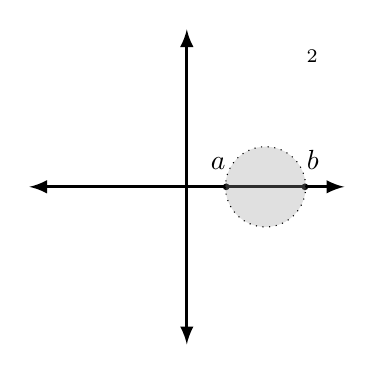
\begin{tikzpicture}
            \draw[latex-latex,very thick] (-2,0)--(2,0);
            \draw[latex-latex,very thick] (0,-2)--(0,2);
            \draw[fill = black] (0.5, 0) circle (1pt);
            \node[above] at (0.4, 0.1) {$a$};
            \draw[fill = black] (1.5, 0) circle (1pt);
            \node[above] at (1.6, 0.1) {$b$};
            \node[] at (1.6, 1.6) {$\RR^2$};
            \draw[dotted, fill = white!60!black, fill opacity=0.3] (1, 0) circle (14.5pt);
        \end{tikzpicture}
    \caption{The interval $(a, b)$ can be viewed as the intersection of $\RR$ with the open disk $N = \set{(x, y) \in \RR^2: \sqrt{(x - \frac{b+a}{2})^2 + y^2} < \frac{b-a}{2}}$, giving rise to a more useful notion of relative openness.}
    \label{fig10}
\end{figure}
\begin{theorem}{}{2.30}
    Let $E \subset Y \subset X$. Then, $E$ is open relative to $Y$ if and only if there exists an open set $G \subset X$ such that $E = G \cap Y$. 
\end{theorem}
\begin{nproof}
    \boxed{\implies} Let $p \in E$. Then, there exists a neighbourhood $N_r^Y(p) \subset E$ (Note that here, $N_r^Y(p) = \set{y \in Y: d(p, y) < r}$). By Theorem \ref{thm:2.24}, we have that $G = \bigcup_{p \in E} N_{r_{p}}^X(p)$ is open. Then, we have that $G \cap Y = \bigcup_{p \in E} N_{r_p}^X(p) \cap Y = \bigcup_{p \in E} N_{r_p}^Y(p) = E$.
    
    \boxed{\impliedby} Suppose $G \subset X$ is open and $E = G \cap Y$. Let $p \in E$. Then, there exists a neighbourhood $N_r^X(p) \subset G$ as $G$ is open, so $N_r^Y(p) = N_r^X(p) \cap Y \subset G \cap Y = E$. Hence, $p$ is an interior point of $E$ in the metric space of $Y$, and hence $E$ is relatively open in $Y$. \qed
\end{nproof}

\subsection{Compactness}
\begin{definition}{Open Covers}{2.31}
    An \textbf{open cover} of a subset $E \subset X$ is a collection $\set{G_\alpha}$ of open sets of $X$ such that $E \subset \bigcup_{\alpha} G_\alpha$.
\end{definition}
\noindent Note that the open cover can be either a finite or infinite (countable or uncountable) collection.
\begin{figure}[htbp]
    \centering
        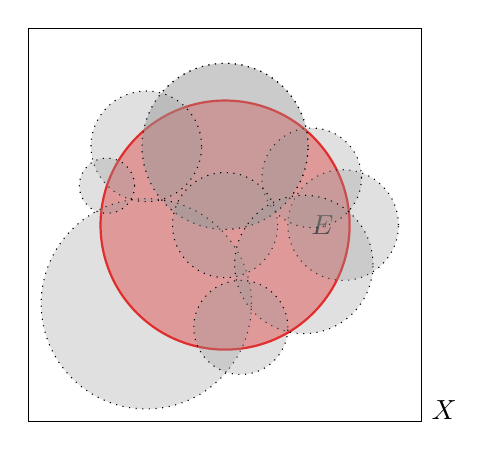
\begin{tikzpicture}
            \draw[red, thick, fill = white!60!red] (0, 0) circle (45pt);
            \node[left] at (1.5, 0) {$E$};
            \draw[] (-2.5, -2.5) -- (-2.5, 2.5) -- (2.5, 2.5) -- (2.5, -2.5) -- (-2.5, -2.5);
            \node[right] at (2.5, -2.35) {$X$};
            \draw[dotted, fill = white!60!black, fill opacity=0.3] (0, 1) circle (30pt);
            \draw[dotted, fill = white!60!black, fill opacity=0.3] (1.5, 0) circle (20pt);
            \draw[dotted, fill = white!60!black, fill opacity=0.3] (1.1, 0.6) circle (18pt);
            \draw[dotted, fill = white!60!black, fill opacity=0.3] (0, 1) circle (30pt);
            \draw[dotted, fill = white!60!black, fill opacity=0.3] (-1, -1) circle (38pt);
            \draw[dotted, fill = white!60!black, fill opacity=0.3] (-1, 1) circle (20pt);
            \draw[dotted, fill = white!60!black, fill opacity=0.3] (-1.5, 0.5) circle (10pt);
            \draw[dotted, fill = white!60!black, fill opacity=0.3] (0, 0) circle (19pt);
            \draw[dotted, fill = white!60!black, fill opacity=0.3] (1, -0.5) circle (25pt);
            \draw[dotted, fill = white!60!black, fill opacity=0.3] (0.2, -1.3) circle (17pt);

    
        \end{tikzpicture}
    \caption{Visualization of a set $E$ and a collection of open disks that form a (finite) open cover of $E$.}
    \label{fig11}
\end{figure}

\begin{definition}{Compactness}{2.32}
    A subset $K \subset X$ is \textbf{compact} if every open cover of $K$ has a finite subcover. Explicitly, if $\set{G_\alpha}$ is an open cover of $K$, then there exist indices $\alpha_1, \ldots, \alpha_n$ such that $K \subset G_{\alpha_1} \cup \ldots \cup G_{\alpha_n}$. 
\end{definition}
\noindent While the above definition might seem strange/esoteric, it turns out to be very useful and important to analysis. We saw in the last lecture that open sets in a sense do not behave ``nicely''; a given set could be open with respect to a subspace $Y$ but not to $X$ (and we had to introduce the notion of relative openness to take care of this fact). Compactness behaves more nicely, as we will see with the following theorem.

\begin{theorem}{}{2.33}
    Suppose $K \subset Y \subset X$. Then, $K$ is compact with respect to $X$ if and only if $K$ is compact with respect to $Y$.
\end{theorem}

\noindent While openness depends on the choice of subspace, this theorem states that compactness is independent of what subspace we choose to look at. It is in a sense an intrinsic property of the set.

\begin{nproof}
    \boxed{\implies} Suppose $K$ is compact with respect to $X$. Let $\set{V_\alpha}$ be an open (in $Y$) cover  of $K$. Then, by Theorem \ref{thm:2.30} we have that there exists $\set{G_\alpha}$ of open sets in $X$ such that $V_\alpha = G_\alpha \cap Y$. Then, $\set{G_\alpha}$ is an open (in $X$) cover of $K$, and hence there exists a finite subcover $K \subset \bigcup_{i=1}^n G_{\alpha_i}$. Then, we have that $K \subset \bigcup_{i=1}^n (G_{\alpha_i} \cap Y) = \bigcup_{i=1}^n V_{\alpha_i}$ which is a finite (sub)cover of $K$ in $Y$. Hence, $K$ is compact with respect to $Y$.
    
    \boxed{\impliedby} Suppose $K$ is compact with respect to $Y$. Let $\set{G_\alpha}$ be an open (in $X$) cover of $K$. Let $V_\alpha = G_\alpha \cap Y$. These are relatively open in $Y$ by Theorem \ref{thm:2.30}, and $\set{V_\alpha}$ still cover $K$. Hence, as $K$ is compact in $Y$, there exists a finite subcover $K \subset \bigcup_{i=1}^n V_{\alpha_i} \subset \bigcup_{i=1}^n G_{\alpha_i}$. Therefore, we have found a finite subcover in $X$, so $K$ is compact in $X$. \qed
\end{nproof}

\begin{theorem}{}{2.34}
    Let $K \subset X$ be compact. Then, $K$ is closed.
\end{theorem}

\noindent A priori, it might seem like the notions of compactness and closedness are quite different, but this theorem shows that they are indeed quite closely related.

\begin{nproof}
    We show that $K^c$ is open. Let $p \in K^c$. For any $q \in K$. Let $r_{q} = \frac{1}{2}d(p, q)$, and define $W_q = N_{r_q}(q)$. So, taking the collection $\set{W_q}$ we have that $\bigcup_{q \in K} W_q$ is an open cover (as it clearly contains every $q \in K$). $K$ is compact, so there exists a finite subcover $\bigcup_{i=1}^n W_{q_i}$. Then, let $r = \min\set{r_{q_1}, \ldots, r_{q_n}}$. Then, $N_r(p) \subset K^c$, hence $p$ is an interior point of $K^c$. Therefore $K^c$ is open, and $K$ is closed by Theorem \ref{thm:2.23}. \qed
\end{nproof}

\begin{theorem}{}{2.35}
    If $F \subset X$ is closed, $K \subset X$ is compact, and $F \subset K$, then $F$ is compact.
\end{theorem}

\begin{nproof}
    Let $\set{V_\alpha}$ be an open cover of $F$. Then, $\set{V_\alpha} \cup F^c$ is an open cover of $K$ ($F^c$ is open as $F$ is closed). Hence, as $K$ is compact, there exists a finite subcover. Dropping $F^c$ (if it is part of the finite subcover of $K$), we obtain a finite subcover of $F$. Hence, $F$ is compact. \qed
\end{nproof}

\begin{ncorollary}{}{}
    If $F \subset X$ is closed and $K \subset X$ is compact, then $F \cap K$ is compact. In other words, compactness is preserved under intersection (with closed sets).
\end{ncorollary}

\begin{nproof}
    If $K$ is compact, it is closed by Theorem \ref{thm:2.34}. $F \cap K$ is closed by Theorem \ref{thm:2.24}, and since $F \cap K \subset K$, by Theorem \ref{thm:2.35} $F \cap K$ is compact. \qed
\end{nproof}

\noindent In a previous course, we may have introduced the definition that compact sets are closed and bounded. Here, we started with a significantly different definition, and work up to prove the Heine-Borel Theorem (coming soon!) which tells us that compactness is equivalent to being closed and bounded in $\RR^k$. Before we move onto such further properties and theorems of compact sets, we may find it useful to consider some examples of sets that are and are not compact.

The singleton set $\set{x}$ is compact in any metric space (out of any open cover, simply pick a single open set that contains $x$; this yields the desired subcover). Moreover, any finite set is compact in any topology (consider that for any open cover of a set of $n$ elements, we can just choose at most $n$ open sets corresponding to each element to form our finite subcover).

Next, consider any infinite set $Y$ in a metric space $X$ with the discrete metric:
\begin{align*}
    d(x, y) = \begin{cases}
        0 & \text{if $x = y$}
        \\ 1 & \text{if $x \neq y$}
    \end{cases}
\end{align*}
Then is $Y \subset X$ compact? The answer is no; consider the open cover of singleton sets, $U = \set{\set{x}: x \in Y}$. First, note that this is indeed an open cover, as $\set{x}$ is open in $X$; consider that $N_r(x) \subset \set{x}$ if $r < 1$, and hence $x$ is an interior point of $\set{x}$, making it open. However, there exists no finite subcover of this open cover as we need to pick an infinite number of singletons to cover each point in $Y$. 


$[1, \infty) \subset \RR$ is not compact as we could consider the open cover $\set{N_1(n): n \in \NN}$, which has no finite subcover. For the sake of contradiction, suppose such a finite subcover existed. Then, there exists some maximum $m$ for which there would be a neighbourhood around in this subcover. Then, all real numbers greater than $m+1$ would not be in this subcover, which is a contradiction. In a similar way, we can show that $\RR \subset \RR, \RR^2 \subset \RR^2$ are not compact. 

Another interesting example to consider is $(0, 1)$. To see that this interval is not compact, consider the open cover $\set{(\frac{1}{n}, 1): n \in \NN}$. This open cover has no finite subcover. Suppose for the sake of contradiction that a finite subcover existed. Then, there would be some minimum $\frac{1}{N}$ such that $(\frac{1}{N}, 1)$ would be in the subcover. But then no $0 < x < \frac{1}{N}$ would be contained in the subcover, which is a contradiction.

From the Heine-Borel theorem, it is clear here that $[1, \infty), \RR, \RR^2$ fail due to the sets being unbounded, and the $(0, 1)$ fails due to the set not being closed. We will now move onto a sequence of Theorems that will eventually lead to Heine-Borel (the climax of this chapter)!

\begin{theorem}{}{2.36}
    Let $\set{K_\alpha}$ is a collection of compact sets such that $\bigcap_{i=1}^n K_{\alpha_{i}} \neq \emptyset$ for any subcollection/any choice of indices $\alpha_1, \ldots, \alpha_n$. Then, $\bigcap_\alpha K_\alpha \neq \emptyset$.
\end{theorem}
\begin{nproof}
    Suppose for the sake of contradiction that the assumptions hold but $\bigcap_\alpha K_\alpha \neq \emptyset$. Pick $\alpha_0$. Then, $K_{\alpha_0} \cap (\bigcap_{\alpha \neq \alpha_0} K_\alpha) = \emptyset$. Hence, $K_{\alpha_0} \subset \left(\bigcap_{\alpha \neq \alpha_0} K_\alpha \right)^c = \bigcup_{\alpha \neq \alpha_0} K_\alpha^c$. Hence, $\set{K_\alpha^c}$ is an open cover of $K_{\alpha_0}$. $K_{\alpha_0}$ is compact, so there exists a finite subcover $\bigcup_{i=1}^n K_{\alpha_i}^c = \left(\bigcap_{i=1}^n K_{\alpha_i}\right)^c$. But then we have that $K_{\alpha_0} \cap \left(\bigcap_{i=1}^n K_{\alpha_i}\right) = \emptyset$, which is a contradiction as a finite intersection should be nonempty by assumption. \qed
\end{nproof}

\begin{ncorollary}{}{}
    Let $\set{K_1, K_2, \ldots}$ be a collection of nonempty and compact sets such that $K_{i+1} \subset K_i$. Then, $\bigcap_{i=1}^\infty K_i \neq \emptyset$.
\end{ncorollary}
\begin{nproof}
    If $n_1 < \ldots < n_m$, then $\bigcap_{i=1}^m K_{n_i} = K_{n_m} \neq \emptyset$. Then, $\bigcap_{i=1}^\infty K_{n_i} \neq \emptyset$ by the above theorem. \qed
\end{nproof}

\begin{theorem}{}{2.37}
    Let $K$ be compact and $E \subset K$ be an infinite set. Then, $E$ has a limit point in $K$.
\end{theorem}
\begin{nproof}
    Suppose for the sake of contradiction that no point of $K$ is a limit point of $E$. Then, for all $q \in K$, then there exists $V_q = N_{r_q}(q)$ such that:
    \begin{align*}
        V_q \cap E = \begin{cases}
            \set{q} & \text{if $q \in E$}
            \\ \emptyset & \text{if $q \notin E$}
        \end{cases}
    \end{align*}
    Trivially, $\set{V_q}$ is an open cover of $K$. So, there exists a finite subcover $\set{V_q}_{i=1}^n$ of $K$. So:
    \begin{align*}
        E \subset K \cap E \subset \left(\bigcup_{i=1}^n V_{q_i}\right) \cap E = \bigcup_{i=1}^n(V_{q_1} \cup E)
    \end{align*}
    But the RHS is a finite set, contradicting the assumption that $E$ is infinite. \qed
\end{nproof}

\subsection{Compactness in \texorpdfstring{$\RR^k$}{Rk} and the Cantor Set}

\begin{theorem}{}{2.38}
    Let $I_n = [a_n, b_n] \subset \RR$ such that $I_{n+1} \subset I_n$ for all $n$. Then, $\bigcap_{i=1}^\infty I_i \neq \emptyset$. 
\end{theorem}
\noindent This theorem is very reminiscent of Theorem \ref{thm:2.37}. However, we cannot apply it directly as we do not know if $[a, b]$ is compact (though we will show that this is indeed the case by the end of the lecture, we want to avoid circular reasoning)!
\begin{figure}[htbp]
    \centering
        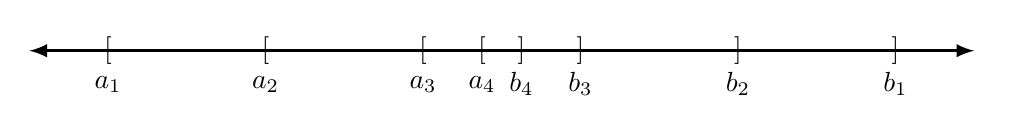
\begin{tikzpicture}
            \draw[latex-latex, very thick] (-6, 0) -- (6,0) node[anchor=south] {$\RR$};
            \node[] at (-5, 0) {$[$};
            \node[below] at (-5, -0.2) {$a_1$};
            \node[] at (5, 0) {$]$};
            \node[below] at (5, -0.15) {$b_1$};
            \node[] at (-3, 0) {$[$};
            \node[below] at (-3, -0.2) {$a_2$};
            \node[] at (3, 0) {$]$};
            \node[below] at (3, -0.15) {$b_2$};
            \node[] at (-1, 0) {$[$};
            \node[below] at (-1, -0.2) {$a_3$};
            \node[] at (1, 0) {$]$};
            \node[below] at (1, -0.15) {$b_3$};
            \node[] at (-0.25, 0) {$[$};
            \node[below] at (-0.25, -0.2) {$a_4$};
            \node[] at (0.25, 0) {$]$};
            \node[below] at (0.25, -0.15) {$b_4$};
        \end{tikzpicture}
    \caption{Visualization of the first few sets $I_n$ in Theorem \ref{thm:2.38}. Note that this is just an example, and the sets do not need to by ``symmetrically shrinking'' around a point as pictured.}
    \label{fig12}
\end{figure}

\begin{nproof}
    We have that $a_n \leq a_{n + m} \leq a_{n + m} \leq b_n$ for all $n, m \in \NN$. Let $E = \set{a_1, a_2, \ldots}$. $E$ is nonempty and bounded by any $b_n$, so by the least upper bound property of $\RR$, there exists $x = \sup E \in \RR$. We then have that $a_n \leq x \leq b_n$ for all $n$ as x is the least upper bound. Hence, $x \in I_n$ for all $n$, and hence $x \in \bigcap_{i=1}^\infty I_i$. We conclude that $\bigcap_{i=1}^\infty I_i \neq \emptyset$. \qed
\end{nproof}

\begin{ndef}{: k-cells}{}
    A \textbf{k-cell} is $I \subset \RR^k$ such that $I = \set{(x_1, x_2, \ldots x_k) \in \RR^k: a_j \leq x_j \leq b_j}$ for some $\set{a_1, \ldots a_j, b_1, \ldots b_j}$.
\end{ndef}
\noindent A $k$-cell can be viewed as the generalization of a rectangle for $\RR^k$.

\begin{theorem}{}{2.39}
    Theorem \ref{thm:2.38} holds for general $k$-cells.
\end{theorem}
\noindent The above theorem follows naturally by applying Theorem \ref{thm:2.38} to each coordinate.

\begin{theorem}{}{2.40}
    Let $I \subset \RR^k$ be a $k$-cell. Then, $I$ is compact.
\end{theorem}

\begin{nproof}
    Lt $\set{G_\alpha}$ be an open cover of $I = I_0$. Suppose for the sake of contradiction that $\set{G_\alpha}$ has no finite subcover. Let $c_j = \frac{1}{2}(a_j + b_j)$. Splitting up $I_0$ along each coordinate (i.e. $[a_j, c_j], [c_j, b_j]$) we obtain $2^k$ $k$-cells $Q_i$, with $I_0 = \bigcup_{i=1}^{2^k}Q_i$. At least one of these $Q_n$s has no finite subcover by assumption. Call this $I_1$. Then, repeat the same division process using $I_1$ (and so on). This yields a sequence of $k$-cells $I_0, I_1, I_2, \ldots$. This sequence has the following properties:
    \begin{enumerate}
        \item $I_0 \supset I_1 \supset I_2 \supset \ldots$
        \item None of $I_n$s have a finite subcover from $\set{G_\alpha}$ by construction.
        \item Let $\delta = \sqrt{\sum_{j=1}^k (b_j - a_j)^2}$ be the diameter of $I$. Then, for $x, y \in I_n$, $\abs{x - y} < 2^{-n}\delta$. 
    \end{enumerate}
    By (a) and Theorem \ref{thm:2.39}, we have that there exists $\v{x}^*$ such that $\v{x}^* \in \bigcap_{n=1}^\infty I_n \subset I$. There exists $\alpha_0$ such that $\v{x} \in G_{\alpha_0}$, and as $G_{\alpha_0}$ is open, there exists some $r > 0$ such that $N_r(\v{x}^*) \subset G_{\alpha_0}$. By (c), we have that $I_n \subset N_{2^{-n+1}\delta}(\v{x}^*)$. For sufficiently large $n$, $I_n \subset  N_{2^{-n+1}\delta}(\v{x}^*) \subset N_r(\v{x}^*) \subset G_{\alpha_0}$, but this contradicts (b). Hence, there must exist a finite subcover of $\set{G_\alpha}$ for $I$. \qed
\end{nproof}

\begin{figure}[htbp]
    \centering
    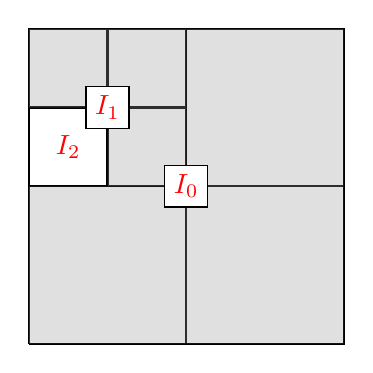
\begin{tikzpicture}
        \draw[thick] (-2, -2) -- (-2, 2) -- (2, 2) -- (2, -2) -- (-2, -2);
        \draw[thick] (0, 2) -- (0, -2);
        \draw[thick] (2, 0) -- (-2, 0);
        \filldraw[fill = white!60!black, opacity = 0.3] (-2, 0) -- (0, 0) -- (0, 2) -- (2, 2) -- (2, -2) -- (-2, -2) -- (-2, 0);
        \draw[thick] (-1, 2) -- (-1, 0);
        \draw[thick] (-2, 1) -- (0, 1);
        \filldraw[fill = white!60!black, opacity = 0.3] (-2, 2) -- (0, 2) -- (0, 0) -- (-1, 0) -- (-1, 1) -- (-2, 1) -- (-2, 2);

        \node[text = red, fill = white, draw] at (0, 0) {$I_0$};
        \node[text = red, fill = white, draw] at (-1, 1) {$I_1$};
        \node[text = red] at (-1.5, 0.5) {$I_2$};
        
    \end{tikzpicture}
    \caption{Visualization of the division process (first three iterations shown) in the proof of Theorem \ref{thm:2.40}, for $I \subset \RR^2$.}
    \label{fig13}
\end{figure}

\begin{theorem}{Heine-Borel}{2.41}
    If a set in $\RR^k$ has the following three properties, then it has the other two.
    \begin{enumerate}
        \item $E$ is bounded and closed.
        \item $E$ is compact.
        \item Every infinite subset of $E$ has at least one limit point in $E$
    \end{enumerate}
    In particular, the equivalence of (a) and (b) is what is commonly referred to as the Heine-Borel theorem.
\end{theorem}
\begin{nproof}
    $\boxed{\text{(a)} \implies \text{(b)}}$ If $E$ is bounded, then there exists a $k$-cell $I$ such that $E \subset I$. $I$ is compact by Theorem \ref{thm:2.40}, and since $E$ is closed, by Theorem \ref{thm:2.35} we have that $E$ is compact.

    $\boxed{\text{(b)} \implies \text{(c)}}$ See Theorem \ref{thm:2.37}.

    $\boxed{\text{(c)} \implies \text{(a)}}$ Suppose first for the sake of contradiction that $E$ is not bounded. Then, $E$ has an infinite subset $S = \set{\v{x}_1,\v{x}_2, \ldots}$ with $\abs{\v{x}_n} > n$ for all $n$. Hence, $S$ has no limit points in $\RR^k$, and therefore no limit points in $E$. But this contradicts (c).

    Suppose next that $E$ is not closed. Then, there exists $\v{x}_0 \in \RR^k$ which is a limit point of $E$ but is not in $E$. Form $S = \set{x_1, x_2, \ldots} \subset E$ with $\abs{x_n - x_0} < \frac{1}{n}$ for all $n$. We now show that $S$ has no limit point in $\RR^k$ except for $\v{x}_0$. To see this, let $\v{y} \in \RR^k, \v{y} \neq \v{x}_0$. Then:
    \begin{align*}
        \abs{\v{x}_n - \v{y}} \geq \abs{\v{x}_0 - \v{y}} - \abs{\v{x}_n - \v{x}_0} \geq \abs{\v{x}_0 - \v{y}} - \frac{1}{n} \geq \abs{\v{x}_0 - \v{y}} - \frac{n}{2}\abs{\v{x}_0 - \v{y}} =  \frac{1}{2}\abs{\v{x}_0 - \v{y}}
    \end{align*}
    Where the last inequality holds for sufficiently large $n$. As every neighbourhood of $\v{y}$ must contain an infinite number of points in $S$ if $\v{y}$ is to be a limit point of $S$ (Theorem \ref{thm:2.20}) we find that $\v{y}$ is not a limit point of $S$. Hence, $S$ has no limit point in $E$, again contradicting (c). We conclude that $E$ must be bounded and closed. \qed
\end{nproof}
\noindent We have already shown that compactness implies closed in any metric space (see Theorem \ref{thm:2.34}). It also turns out that compactness implies boundedness in any metric space, as well!
\begin{proof}
    Let $E \subset X$ be compact. Suppose for the sake of contradiction that $E$ was unbounded. Pick any $x_0 \in E$, then $E$ is unbounded, so $\left(N_n(x_0)\right)^c \cap E \neq \emptyset$ for all $n \in \NN$. But, $E \subset \bigcup_{n \in \NN} N_n(x_0)$, and hence $\set{N_n(x_0)}$ forms an (infinite) subcover of $E$. By the compactness of $E$, there exists a finite subcover; but then, there is a maximal radius neighbourhood of $x_0$ that is contained in this subcover. However, this neighbourhood would not contain all $x \in E$ as $E$ is unbounded, which is a contradiction.
\end{proof}
\noindent From this, we have shown that compact implies closed and bounded in any metric space (i.e. the forwards direction of Heine-Borel holds in general). The converse is not always true, however. For one example, consider any infinite set $E$ in a metric space equipped with the discrete metric. $E$ is closed, since $E$ has no limit points (the neighbourhood of radius $r \leq 1$ around any point contains no other point of $E$). $E$ is bounded as a neighbourhood of radius $r > 1$ around any point contains all points of $E$. However, as we have discussed previously, $E$ is not compact. Another example would be $\RR^\infty$ (i.e. the set of all infinite sequences of real numbers), but the argument for this is left as homework (HW5). 


\begin{theorem}{Weierstrauss}{2.42}
    Suppose $E \subset \RR^k$ is bounded and infinite. Then, $E$ has a limit point in $\RR^k$.
\end{theorem}
\begin{nproof}
    Since $E$ is bounded, $E \subset I \subset \RR^k$ for some $k$-cell $I$. By Theorem \ref{thm:2.40} $E$ is compact, so by Theorem \ref{thm:2.37} $E$ has a limit point in $I$ (and hence in $\RR^k$). \qed
\end{nproof}

\noindent Having proven the landmark (Heine-Borel) theorem of this section, we close this chapter with discussion of perfect sets and the Cantor set.
\setcounter{rudin}{17}
\begin{definition}{Perfect Sets}{2.18h}
    A set $P \subset X$ is \textbf{perfect} if $P$ is closed and every point of $P$ is a limit point of $P$. 
\end{definition}

\setcounter{rudin}{42}
\begin{theorem}{}{2.43}
    Let $P \subset \RR^k$ be nonempty and perfect. Then, $P$ is uncountable.
\end{theorem}
\begin{nproof}
    Since $P$ has limit points, it is not finite by Theorem \ref{thm:2.20}. Assume for the sake of contradiction that $P$ is countable. Then, $P = \set{\v{x}_1, \v{x}_2, \ldots}$. Let $V_1 = N_r(\v{x_1})$ be any neighbourhood of $\v{x}_1$. Suppose we construct $B_n$ such that $V_n \cap P \neq \emptyset$ (note that we don't assume that $\v{x}_n \in V_n$, just that some point $\v{p} \in P$ is in $V_n$). Since $P$ is perfect, we may construct $V_{n+1}$ such that:
    \begin{enumerate}[(i)]
        \item $\overline{V}_{n+1} \subset V_n$
        \item $\v{x}_n \notin \overline{V}_{n+1}$
        \item $V_{n+1} \cap P \neq \emptyset$
    \end{enumerate}
    Note that $\overline{V}_{n}$ is closed and bounded, and hence is compact by Theorem \ref{thm:2.41}. Hence, by the corollary to Theorem \ref{thm:2.35} we have that $K_n = \overline{V}_n \cap P$ is also compact. By (ii), we have that $\v{x}_n \notin \bigcap_{n=1}^\infty K_n$, and this holds for all $n \in \NN$. Hence, $P \cap \bigcap_{n=1}^\infty K_n = \emptyset$, but $K_n \subset P$, so it follows that $\bigcap_{n=1}^\infty K_n = \emptyset$. But $K_n$ is non-empty, compact, and $K_{n+1} \subset K_n$, so this contradicts the corollary to Theorem \ref{thm:2.36}. We conclude that $P$ is uncountable. \qed
\end{nproof}

\begin{ncorollary}{}{}
    Every interval $[a, b]$ is uncountable. It follows that $\RR$ is uncountable.
\end{ncorollary}

\begin{definition}{The Cantor Set}{2.44}
    Let $E_0 = [0, 1]$. Then, remove the middle third (that is, $(\frac{1}{3}, \frac{2}{3})$) to obtain $E_1 = [0, \frac{1}{3}]\cup[\frac{2}{3}, 1]$. Then remove the middle thirds of each of these parts to get $E_2 = [0, \frac{1}{9}]\cup[\frac{2}{9}, \frac{1}{3}]\cup[\frac{2}{3}, \frac{7}{9}]\cup[\frac{8}{9}, 1]$. This yields a sequence of sets $E_0 \supset E_1 \supset E_2 \supset E_3 \supset \ldots$.

    Then, we may define the \textbf{Cantor set} as $P = \bigcap_{n=1}^\infty E_n$. 
\end{definition}
\noindent Although we will rigorously define a measure in this course, each $E_n$ in the above construction is the union of $2^n$ intervals of measure $\frac{1}{3^n}$, for a total measure of $\frac{2^n}{3^n}$ for each $E_n$. Taking the limit of $n \rightarrow \infty$, we can therefore see that the Cantor set has measure zero. However, the Cantor set is uncountable (as we will see shortly), making it an example of an uncountable set of measure zero.

\begin{figure}[htbp]
    \centering
    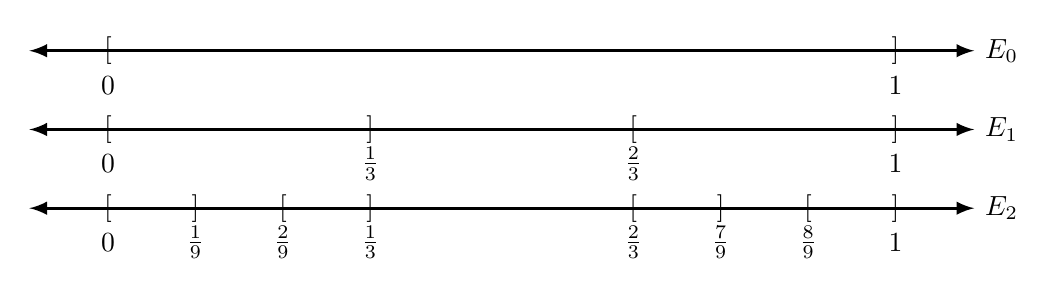
\begin{tikzpicture}
        \draw[latex-latex, very thick] (-6, 1) -- (6,1) node[anchor=west] {$E_0$};
        \node[] at (-5, 1) {$[$};
        \node[below] at (-5, 0.8) {$0$};
        \node[] at (5, 1) {$]$};
        \node[below] at (5, 0.8) {$1$};
        \draw[latex-latex, very thick] (-6, 0) -- (6, 0) node[anchor=west] {$E_1$};
        \node[] at (-5, 0) {$[$};
        \node[below] at (-5, -0.2) {$0$};
        \node[] at (-1.67, 0) {$]$};
        \node[below] at (-1.67, -0.1) {$\frac{1}{3}$};
        \node[] at (1.67, 0) {$[$};
        \node[below] at (1.67, -0.1) {$\frac{2}{3}$};
        \node[] at (5, 0) {$]$};
        \node[below] at (5, -0.2) {$1$};
        \draw[latex-latex, very thick] (-6, -1) -- (6,-1) node[anchor=west] {$E_2$};
        \node[] at (-5, -1) {$[$};
        \node[below] at (-5, -1.2) {$0$};
        \node[] at (-3.89, -1) {$]$};
        \node[below] at (-3.89, -1.1) {$\frac{1}{9}$};
        \node[] at (-2.78, -1) {$[$};
        \node[below] at (-2.78, -1.1) {$\frac{2}{9}$};
        \node[] at (-1.67, -1) {$]$};
        \node[below] at (-1.67, -1.1) {$\frac{1}{3}$};
        \node[] at (1.67, -1) {$[$};
        \node[below] at (1.67, -1.1) {$\frac{2}{3}$};
        \node[] at (2.78, -1) {$]$};
        \node[below] at (2.78, -1.1) {$\frac{7}{9}$};
        \node[] at (3.89, -1) {$[$};
        \node[below] at (3.89, -1.1) {$\frac{8}{9}$};
        \node[] at (5, -1) {$]$};
        \node[below] at (5, -1.2) {$1$};
    \end{tikzpicture}
    
    \caption{Visualization of the first few sets $E_0, E_1, E_2$ used in the construction of the Cantor set.}
    \label{fig14}
\end{figure}

\begin{ntheorem}{}{}
    The Cantor set contains no interval $(a, b)$.
\end{ntheorem}
\begin{nproof}
    (Sketch) Any interval $(a, b)$ contains some interval $\left(\frac{3k+1}{3^m}, \frac{3k+2}{3^m}\right)$ which are all removed in the construction of the set. \qed
\end{nproof}
\noindent If the Cantor set contains no intervals, then how is it uncountable? It might help to consider that by construction, the endpoints of each $E_n$ belong to $P$; in the limit, this yields an uncountable number of points contained in $P$. 

\begin{ntheorem}{}{}
    The Cantor set is uncountable. Moreover, it is perfect.
\end{ntheorem}


\begin{nproof}
    Let $X \in P$ and $S$ be an interval such that $x \in S$. Let $I_n$ be the interval of $E_n$ containing $x$. The length of $I_n$ is given by $\frac{1}{3^n}$. For sufficiently large $n$, $I_n \subset S$. Let $x_n$ be an endpoint of $I_n$ such that $x_n \neq x$. By construction, $x_n \in P$, and hence $x$ is a limit point of $P$ by construction. Additionally, $P$ is closed by Theorem \ref{thm:2.24} as it is an infinite intersection of closed sets. Hence $P$ is perfect, and by Theorem \ref{thm:2.43} it is uncountable. \qed
\end{nproof}

\subsection{Connected Sets}
Though not covered in lecture, we here briefly discuss connectedness as it comes up later in Chapter 4.

\begin{definition}{Connected Sets}{2.45}
    Two subsets $A, B$ of a metric space $X$ are separated if $A \cap \overline{B} = \overline{A} \cap B = \emptyset$. A set $E \subset X$ is connected if $E$ is not a union of two nonempty separated sets.
\end{definition}
\noindent Separated sets are disjoint, but disjoint sets are not necessarily separated; for example, $A = [0, 1]$ and $B = (1, 2)$ are not separated as $\overline{B} = [1, 2]$ and hence $A \cap \overline{B} = \set{1}$. However, $A = (0, 1)$ and $B = (1, 2)$ are separated. The following theorem characterizes connected subsets of $\RR$. 
\setcounter{rudin}{46}
\begin{theorem}{}{2.47}
    A subset $E \subset \RR$ is connected if and only if it has the property that if $x, y \in E$ and $x < z < y \in E$, then $z \in E$.
\end{theorem}
\begin{nproof}
    Not covered in lecture, see Rudin.
\end{nproof}
